\section{Hiện thực hệ thống}
Trong phần này, chúng tôi xin trình bày chi tiết về kỹ thuật cách rút trích các đặc trưng, hiện thực bộ phân loại cũng như tích hợp các yếu tố đó vào hệ thống. 
Chúng tôi hiện thực hệ thống bằng ngôn ngữ lập trình Python, phiên bản 2.7

\subsection{Thư viện sử dụng}
Chúng tôi sử dụng các thư viện: NLTK và Scikit-learn, cùng một số thư viên khác. Tất cả các thư viện đều là mã nguồn mở và miễn phí.
\subsubsection*{NLTK}
NLTK \cite{bird2009natural} là một \term{platform} xây dựng trên ngôn ngữ lập trình Python, cung cấp các công cụ để thao tác với văn bản. NLTK tích hợp hơn 50 \term{corpora} và các nguồn từ vựng (\term{lexicon}) như WordNet, SentiWordNet cùng các thư viện để xử lý ngôn ngữ tự nhiên, hỗ trợ: \term{tokenization}, \term{stemming}, \term{lemmination}, \term{parsing}. Ngoài ra NLTK đóng gói và cung cấp các giao diện lập trình (\term{API}) của các thư viện khác (thư viện Stanford NLP).\\

Trong nghiên cứu này, chúng tôi sử dụng NLTK như công cụ chính để thực hiện các bước tiền xử lý: tách câu, \term{tokenization}, \term{stemming}, \term{lemmination}
\subsubsection*{Scikit-learn}
Scikit-learn \cite{scikit-learn} là bộ thư viện về lĩnh vực Học máy trên nền tảng thư viện SciPy, sử dụng ngôn ngữ lập trình Python. Thư viện này cung cấp rất nhiều công cụ mà một bài toán Học máy cần dùng: Các giải thuật phân loại, hồi quy, phân cụm, \ldots; các công cụ tiền xử lý; các giải thuật thu giảm chiều; và các công cụ giúp lựa chọn, đánh giá mô hình.\\

Trong nghiên cứu này, chúng tôi sử dụng Scikit-learn là công cụ chính để hiện thực đặc trưng N-gram và giải thuật học máy SVM.

\subsubsection*{Các thư viện khác}
Ngoài 2 thư viện kể trên, chúng tôi sử dụng thêm:
\begin{itemize}
\item[•] NumPy giúp thao tác trên dữ liệu dạng vector.
\item[•] Pandas giúp đọc file, viết file và quản lý tập dữ liệu huấn luyện và dữ liệu để đánh giá.
\end{itemize}
\subsection{Hiện thực rút trích đặc trưng}
Trong phần này, chúng tôi sẽ trình bày cách thức hiện thực để từ một câu văn chuyển thành một vector, hoặc từ danh sách các câu chuyển thành một mảng 2 chiều. Từ đó làm input cho giải thuật học máy SVM
\subsubsection*{Đặc trưng N-gram}
Scikit-learn cung cấp các công cụ để làm việc với dữ liệu dạng text. Trong số này, chúng tôi sử dụng module sklearn.feature\_extraction.text.CountVectorizer để hiện thực đặc trưng N-gram. Như mô tả ở mục \ref{sec:ngram}, n-gram được trích xuất qua 2 bước:\\

Bước đầu tiên: Xây dựng tập từ vựng T. Scikit-learn cung cấp lớp CountVectorizer cho tác vụ này.
\begin{lstlisting}
vectorizer = CountVectorizer(input, min_df, binary, ngram_range)
\end{lstlisting}
Hàm khởi tạo CountVectorizer cung cấp 17 tham số, tuy nhiên, trong nghiên cứu này chúng tôi chỉ quan tâm đến 4 tham số, các tham số còn lại sử dụng giá trị mặc định:
\begin{description}
\item[input] Là các câu trong tập dữ liệu huấn luyện
\item[min\_df] Là số nguyên thể hiện số câu câu ít nhất chứa n-gram để n-gram đó được thêm vào tập từ vựng. Tham số này đã được giải thích chi tiết tại \ref{sec:ngram}
\item[binary] Là giá trị True hoặc False. Nếu $binary=True$, giải thuật sử dụng \term{vector nhị phân}\footnotemark, \footnotetext{2 khái niệm này được định nghĩa tại Mục \ref{sec:ngram}, phần Rút trích}
ngược lại sử dụng \term{vector số nguyên}\footnotemark
 \footnotetext{2 khái niệm này được định nghĩa tại Mục \ref{sec:ngram}, phần Rút trích}
 \item[ngram\_range] Là một \term{tuple}, có dạng $(a, b)$. Giải thuật sẽ sử dụng các loại n-gram từ a-gram đến b-gram. \\
 Ví dụ $ngram\_range = (1,3)$: Giải thuật sử dụng 3 loại n-gram: Uni-gram, bi-gram và tri-gram.
\end{description}

Bước thứ 2: xây dựng tập vector đại diện cho mỗi câu trong tập huấn luyện. Bước này được thực hiện bằng cách gọi hàm:
\begin{lstlisting}
vectors-ngram = vectorizer.transform(raw_documents).toarray()
\end{lstlisting}
trong đó $raw\_documents$ là tập hợp các câu. Hàm trên trả về một mảng 2 chiều $n*m$ với n là số lượng câu trong tập $raw\_documents$ và $m$ là kích thước của tập từ vựng
\subsubsection*{Đặc trưng Chang phrase}
Đặc trưng Change phrase ánh xạ một câu sang 1 vector 4 chiều. Trong phần hiện thực, chúng tôi định nghĩa hàm training\_change\_phrase:
\begin{lstlisting}
def training_change_phrase(raw_documents):
\end{lstlisting}
Hàm trả về mảng 2 chiều $n*4$ với $n$ là số lượng câu trong tập $raw\_documents$
\subsubsection*{Đặc trưng phủ định}
Chúng tôi sử dụng đồng thời 2 công cụ để trích xuất đặc trưng phủ định: Metamap và NegEx. Việc này nhằm so sánh hiệu quả của 2 công cụ trên và chọn ra công cụ phù hợp hơn đối với nghiên cứu này.
\subsubsection*{SO-CAL}
Trong phần này, chúng tôi sử dụng phiên bản hiện thực của nghiên cứu \cite{taboada2011lexicon}. Nhóm tác giả của nghiên cứu \cite{taboada2011lexicon} đã hiện thực công cụ online để tính điểm số cho 1 đoạn văn, giao diện được mô tả như Hình \ref{fig:socal}.
\begin{figure}
\centering
\begin{subfigure}[b]{0.4\textwidth}
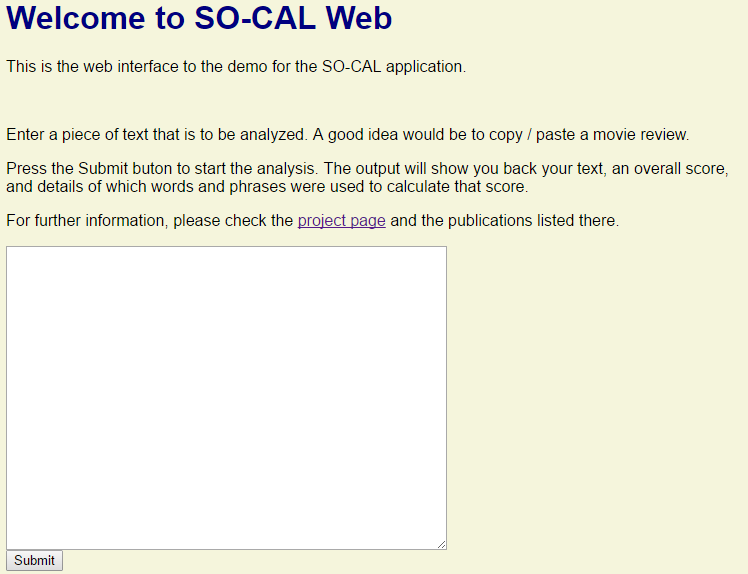
\includegraphics[scale=0.3]{../hinh/socal.png}
\caption{Nhập 1 đoạn text sau đó nhấp submit để chuyển đến trang kết quả}
\end{subfigure}
~
\begin{subfigure}[b]{0.4\textwidth}
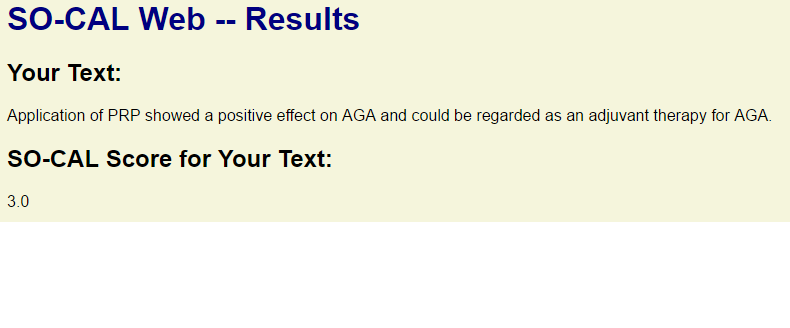
\includegraphics[scale=0.3]{../hinh/socal_result.png}
 \caption{Giao diện kết quả}
\end{subfigure}
\caption{Công cụ online để tính điểm SO-CAL} \label{fig:socal}
\end{figure}

Để tích hợp vào hệ thống, nhóm sử dụng package re trong Python, sử dụng phương thức HTTP POST để gửi yêu cầu lên trang web, sau đó parse phần kết quả trả về để lấy ra thông tin điểm số.
\subsection{Hiện thực bộ phân loại SVM}
\begin{figure}[H]
\centering
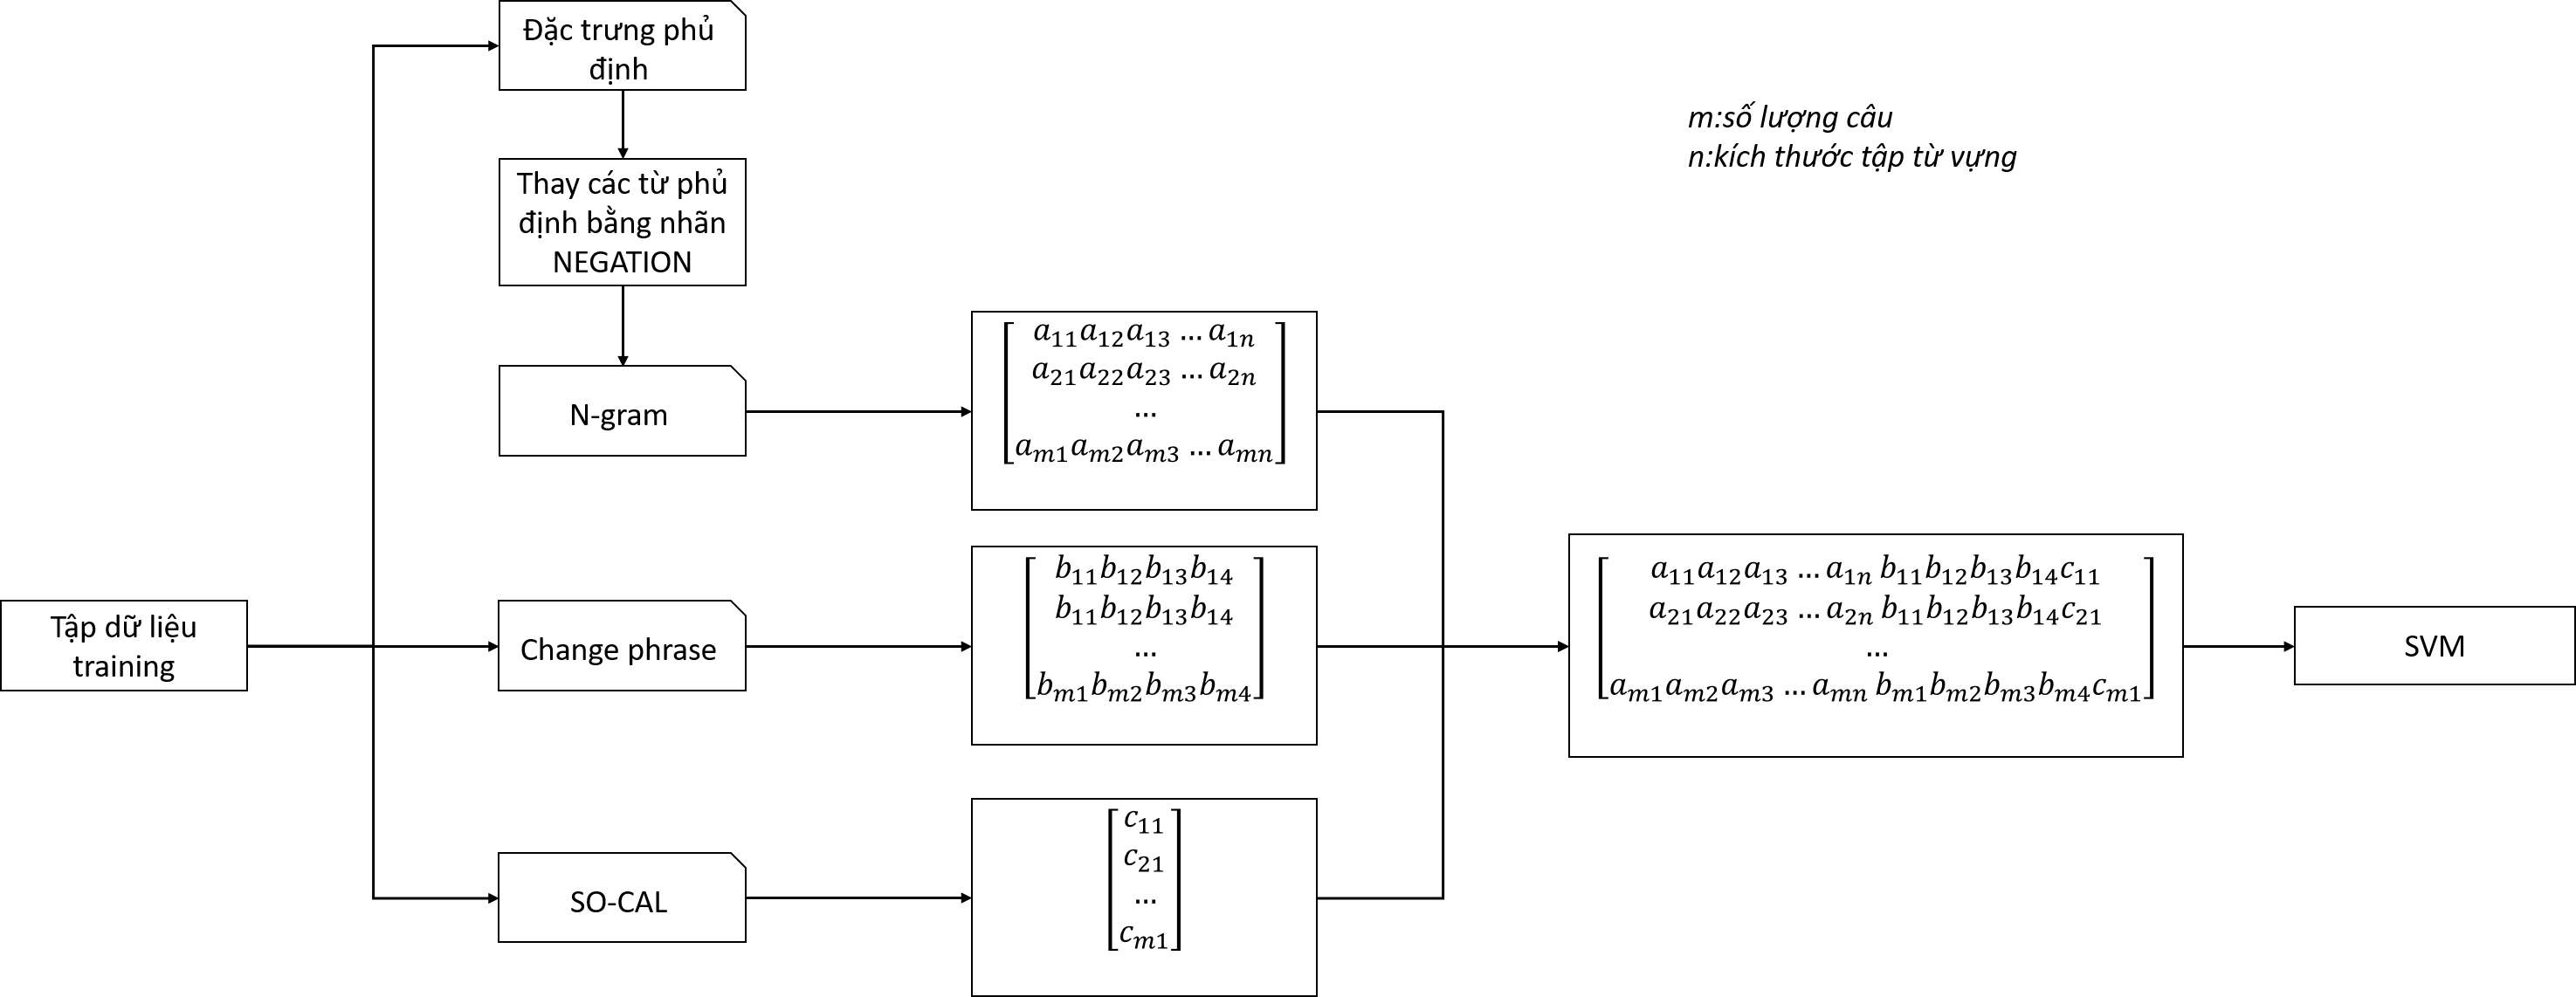
\includegraphics[scale=0.3]{../hinh/ket_hop_dac_trung.png}
\caption{Kết hợp các đặc trưng trước khi đưa vào SVM huấn luyện} \label{fig:ket-hop-dac-trung}
\end{figure}
Các đặc trưng sau khi được rút trích như đã mô tả sẽ được kết hợp lại để với mỗi câu, chỉ có 1 vector đại diện. Mô hình kết hợp các đặc trưng được miêu tả như Hình \ref{fig:ket-hop-dac-trung}

Chúng tôi sử dụng lớp SVM.SVC của thư viện Scikit-learn để hiện thực giải thuật học máy SVM.\\
\begin{minipage}{0.95\textwidth}
\begin{lstlisting}
clf = svm.SVC(decision_function_shape = 'ovr', C = c,           kernel = 'rbf', class_weight = 'balanced')
clf.fit(data_x, data_y)
\end{lstlisting}
\end{minipage}

Hàm khởi tạo SVM.SVC ở dòng 1 có các tham số được sử dụng như sau:
\begin{description}
\item[decision\_function\_shape] Định nghĩa cách SVC hiện thực bộ phân loại đa lớp. Nếu decision\_function\_shape='ovr' (one-vs-rest), SVC tạo ra 3 hàm quyết định (decision function): Một câu có thuộc lớp \tichcuc hay không, một câu có thuộc lớp \tieucuc hay không và một câu có thuộc lớp \trungtinh hay không. Nếu decision\_function\_shape='ovo' (one-vs-one), SVC tạo ra 3 hàm quyết định: Một câu thuộc lớp \tichcuc hay thuộc lớp \tieucuc, một câu thuộc lớp \tieucuc hay thuộc lớp \trungtinh và một câu thuộc lớp \trungtinh hay thuộc lớp \tichcuc
\item[C] là hệ số được định nghĩa trong mô hình soft-margin của giải thuật SVM. Hệ số này đánh đổi giữa việc chấp nhận 1 vài dữ liệu bị phân loại sai, bù lại việc mặt phẳng hàm quyết định (decision surface) trở nên phức tạp, ít tuyến tính. C cao thì SVC càng phân loại chính xác các dữ liệu trong tập huấn luyện, ngược lại C thấp thì mặt phẳng hàm quyết định càng đơn giản.
\item[kernel] Định nghĩa loại \term{kernel} SVC sử dụng: linear, poly, rbf, sigmoid, precomputed
\item[class\_weight] Tùy chọn cách xử lý khi số lượng các lớp trong tập huấn luyện bị chêch lệch
\end{description}

Sau khi khởi tạo, hàm clf.fit(data\_x, data\_y) được gọi với data\_x là dữ liệu tập huấn luyện sau khi đã qua các bước rút trính đặc trưng để ánh xạ từ 1 câu sang 1 vector, data\_y là vector chứa nhãn tương ứng.